\documentclass[sigconf,natbib=false]{acmart}
%%
%% \BibTeX command to typeset BibTeX logo in the docs
\AtBeginDocument{%
  \providecommand\BibTeX{{%
    \normalfont B\kern-0.5em{\scshape i\kern-0.25em b}\kern-0.8em\TeX}}}

%% Rights management information.  This information is sent to you
%% when you complete the rights form.  These commands have SAMPLE
%% values in them; it is your responsibility as an author to replace
%% the commands and values with those provided to you when you
%% complete the rights form.
\setcopyright{acmlicensed}
\copyrightyear{2025}
\acmYear{2025}
\acmDOI{XXXXXXX.XXXXXXX}

%% These commands are for a PROCEEDINGS abstract or paper.
\acmConference[ACM REP'25]{2025 ACM Conference on Reproducibility and Replicability}{July 29-31, 2025}{Vancouver, Canada}
%
%  Uncomment \acmBooktitle if th title of the proceedings is different
%  from ``Proceedings of ...''!
%
%\acmBooktitle{Woodstock '18: ACM Symposium on Neural Gaze Detection,
%  June 03--05, 2018, Woodstock, NY} 
\acmISBN{978-1-4503-XXXX-X/18/06}

\usepackage{tcolorbox}
\tcbuselibrary{theorems}
\usepackage{cleveref}
\newtcbtheorem[]{trap}{Pitfall}{colback=black!5,colframe=black!35,fonttitle=\bfseries}{th}
\newtcbtheorem[]{lesson}{Takeaway}{colback=black!5,colframe=black!35,fonttitle=\bfseries}{th}
\newcommand{\repro}{reproducibility}
\newcommand{\Repro}{Reproducibility}
\newcommand{\transpo}{\emph{Transposition}}
\newcommand{\flavour}{\emph{flavour}}
\newcommand{\flavours}{\emph{flavours}}
\newcommand{\ie}{\emph{i.e.,}}
\newcommand{\eg}{\emph{e.g.,}}
\newcommand{\nix}{\emph{Nix}}
\newcommand{\nixos}{\emph{NixOS}}
\newcommand{\nxc}{\emph{NixOS Compose}}
\newcommand{\enos}{\emph{EnOSlib}}
\newcommand{\grid}{\emph{Grid'5000}}
\newcommand{\kam}{\emph{Kameleon}}
\newcommand{\kad}{\emph{Kadeploy}}
\newcommand{\mel}{\emph{Melissa}}
\newcommand{\store}{\emph{Nix Store}}
\newcommand{\ad}{Artifact Description}
\newcommand{\aeval}{Artifact Evaluation}
\newcommand{\adae}{\ad/\aeval}
\newcommand{\df}{\texttt{Dockerfile}}
\newcommand{\todo}[1]{{\color{red}{TODO: #1}}}
\usepackage{hyperref}
\usepackage{array}
\usepackage{caption}
\usepackage{subcaption}
\usepackage{graphicx}
\usepackage{siunitx}
%\usepackage[table]{xcolor}
\usepackage{multirow}
\usepackage{hhline}
\usepackage{calc}
%\usepackage{tabularx}
\usepackage{fontawesome}
\usepackage[para,online,flushleft]{threeparttable}
\usepackage{booktabs}
\usepackage{longtable}
\usepackage{amsmath,amsfonts}
\usepackage{textcomp}
\usepackage{listings}
\definecolor{commentcolour}{rgb}{0.04,0.43,0.17}
\definecolor{keywordcolour}{rgb}{0.65,0.15,0.64}
\definecolor{backcolour}{rgb}{1,1,1}
\definecolor{linenumbercolour}{rgb}{0.1,0.1,0.1}
\definecolor{stringcolour}{rgb}{0.56,0.06,0.49}
\lstdefinestyle{mystyle}{
  backgroundcolor=\color{backcolour},   
  commentstyle=\color{commentcolour},
  keywordstyle=\color{keywordcolour},
  numberstyle=\tiny\color{linenumbercolour},
  stringstyle=\color{stringcolour},
  basicstyle=\ttfamily\footnotesize,
  breakatwhitespace=false,         
  breaklines=true,                 
  captionpos=b,                    
  keepspaces=true,                 
  numbers=left,                    
  numbersep=5pt,                  
  showspaces=false,                
  showstringspaces=false,
  showtabs=false,                  
  tabsize=2,
  framexrightmargin=-12pt
}
\lstset{style=mystyle, frame=single}

%\usepackage[backend=biber,style=trad-abbrv,firstinits=true]{biblatex}
\usepackage[
  datamodel=software,
  style=trad-abbrv,
  backend=biber
]{biblatex}
\addbibresource{references.bib}
\usepackage{software-biblatex}

\begin{document}

\title{%
  (Very) Preliminary Study of the Longevity of Docker Images from Research Artifacts
}

\author{Quentin Guilloteau}
\email{quentin.guilloteau@inria.fr}
\affiliation{%
  \institution{INRIA}
  \country{France}
}

% \renewcommand{\shortauthors}{Trovato and Tobin, et al.}

%%
%% The abstract is a short summary of the work to be presented in the
%% article.
\begin{abstract}
  todo
\end{abstract}

%% %% The code below is generated by the tool at http://dl.acm.org/ccs.cfm.
%% Please copy and paste the code instead of the example below.
%%
\begin{CCSXML}
<ccs2012>
 <concept>
  <concept_id>00000000.0000000.0000000</concept_id>
  <concept_desc>Do Not Use This Code, Generate the Correct Terms for Your Paper</concept_desc>
  <concept_significance>500</concept_significance>
 </concept>
 <concept>
  <concept_id>00000000.00000000.00000000</concept_id>
  <concept_desc>Do Not Use This Code, Generate the Correct Terms for Your Paper</concept_desc>
  <concept_significance>300</concept_significance>
 </concept>
 <concept>
  <concept_id>00000000.00000000.00000000</concept_id>
  <concept_desc>Do Not Use This Code, Generate the Correct Terms for Your Paper</concept_desc>
  <concept_significance>100</concept_significance>
 </concept>
 <concept>
  <concept_id>00000000.00000000.00000000</concept_id>
  <concept_desc>Do Not Use This Code, Generate the Correct Terms for Your Paper</concept_desc>
  <concept_significance>100</concept_significance>
 </concept>
</ccs2012>
\end{CCSXML}

\ccsdesc[500]{Do Not Use This Code~Generate the Correct Terms for Your Paper}
\ccsdesc[300]{Do Not Use This Code~Generate the Correct Terms for Your Paper}
\ccsdesc{Do Not Use This Code~Generate the Correct Terms for Your Paper}
\ccsdesc[100]{Do Not Use This Code~Generate the Correct Terms for Your Paper}

%%
%% Keywords. The author(s) should pick words that accurately describe
%% the work being presented. Separate the keywords with commas.
\keywords{Reproducibility, Artifact Evaluation, Badges, Lifetime}

\received{12 February 2024}
\received[revised]{12 March 2009}
\received[accepted]{5 June 2009}

%%
%% This command processes the author and affiliation and title
%% information and builds the first part of the formatted document.
\maketitle

%% PAPER STARTS HERE -----------------------------------------------------------------------------------------------

\section{Introduction}

% \todo{split into intro and related work?}
% 
% \begin{itemize}
% \item Reproducibility crisis \cite{baker500ScientistsLift2016}
% \item Also in computer science \cite{collberg_repeatability_2015}, but most impact is from the missing environment.
% \item Artifact evaluation in conferences \cite{kidwell2016badges}
% \item Software environment is a problem/difficul aspect \cite{mytkowicz_producing_nodate}
% \item conferences recommand to use containers to share the software environmnent,
% \item more and more papers are linking code \cite{paperswithcode, kang2023papers, hong2013software}
% \item a lot of papers proposing solution around virtualisation and container \cite{brammer2011paper, brinckman2019computing}
% \item but container recipes are based on non-reproducibile tools (package managers and bad practices) \cite{guilloteau2024longevity, guilloteau2024frustrations}
% \item even though Nix \cite{dolstra_nix_2004} and Guix \cite{courtes_functional_2013} already very good solutions but not used enough \cite{guilloteau2024longevity}
% \item trade-off between storing the result of the image builts by the authors and the recipe \cite{software_heritage_2017, zenodo, figshare}
% \item we need the dev environment to \emph{inspect} and introduce \emph{variation} \cite{mercier2018considering}. \cite{blinry, nvidia_cuda_lifetime}
% \end{itemize}

The entire scientific community has been struck by the ``Reproducibility Crisis''~\cite{baker500ScientistsLift2016}, and Computer Science does not make exception~\cite{collberg_repeatability_2015}.
In order to improve the reproducibility of articles in Computer Science, the community set up \adae\ processes~\cite{kidwell2016badges} where authors would submit (if they want) the artifact required to reproduced the main results from their article.
Then a set of artifact reviewers would try to reproduce those main results given the artifact from the authors.
Based on the result of the reproduction attempt, the article is then awarded \emph{badges} to promote its reproducibility aspect.
The link to the artifacts can be found in the published version of the article, sometimes with an appendix giving more information about the artifact (\eg\ download instructions, hardware requirements, experiments workflow) \cite{paperswithcode, kang2023papers, hong2013software}.

One difficult aspect of creating a truly reproducible artifact is to properly control the software environment: packages and libraries versions.
Several works already shed light on the possible varability of results given a badly captured software environment \cite{mytkowicz_producing_nodate} \todo{more}.
To tackle this issue, the conference \ae\ committees have been pushing the authors to provide containers or virtual machines to share their artifacts in order to ``freeze'' their software environment.
However, authors generate their artifact right before the artifact submission~\cite{guilloteau2024longevity, guilloteau2024frustrations}.
Moreover, in the case of usual virtualisation techiniques to generate containers or virtual machines, users have to write the recipe made of a list of commands to execute from a base image.
This approach has several limitations.
First, these base images can vary, either because of bad practices from the users (\eg\ using the \texttt{latest} version of the images) or from the administrators of the image (\eg\ pushing a different image to a previously defined tag).
These base images can also be removed by the administrators making all the recipes unbuildable~\cite{nvidia_cuda_lifetime}.
Another limitation of this approach is the heavy dependency on non-reproducible tools such as classical package managers (\eg\ \texttt{apt}, \texttt{dpkg}, \texttt{yum}).
Hence, rebuilding a recipe of a container or a virtual machine can yield different results, and thus ``breaking'' the reproducibility of the results.
One solution would be to store the container itself (\ie\ the tarball) onto some long term storage for example Zenodo~\cite{zenodo}.
But this come with the downside of requiring more storage space than just storing the recipe (binary vs. text file).
This practice has thus some \textbf{severe scalability issues in terms of longevity}.
Moreover, storing the built binary image exhibits limitations when needed to \emph{inspect} the actual content of the image, and when a modification of the software environment capture by this image is needed~\cite{mercier2018considering}.
Having the opportunity to extend previous scientific work \todo{...}

A better solution would be to use tools such as Nix~\cite{dolstra_nix_2004} or Guix~\cite{courtes_functional_2013} which are focused on reproducibility and which are able to rebuild the \emph{exact same} software environment from a textual description and with longevity properties~\cite{courtes2024source}, but these tools are unfortunately poorly adopted by the community~\cite{guilloteau2024longevity}.

\subsection{Research Questions}


This paper proposes a framework to evaluate the variations in resulting software environment produced by \texttt{Dockerfile}s from research artifacts.
We show initial results from five \texttt{Dockerfile}s built every month for six months.

In this paper, we build Docker images coming from five artifacts of the EuroPar'24 conference.
We built each image on 6 dates.


We aim to answer the following questions:

\begin{enumerate}
\item How does the packages evolve through time when captured in a \texttt{Dockerfile}?
\item Which packaging tool is the most victim to variation in its resulting software environment?
\item Which are the most volatile packages?
\item Which practices in \df s are the most damaging to reproducibility?
\end{enumerate}


The goal is not to dunk on authors or conferences, but simply to exhibit the potential issues with \texttt{Dockerfile}s.

\newpage
\section{Framework}

\begin{itemize}
\item `ecg`, Python tool, Licence, lines of code
\item architecture (nickel, what is supported)
\item process (submit new artifacts)
\item end goal of the project
\end{itemize}

\subsection{Artifact representation}

An \df\ from an artifact is represented as a Nickel \cite{nickel} file.
This Nickel file is then \emph{verified} against the contract (\todo{link to contract}) and translated to a JSON file fed to \texttt{ecg}.

\begin{lstlisting}[caption=Example of Artifact representation in Nickel format.]
{
  version = "1.0",
  artifact_url = "https://zenodo.org/.../artifact.zip",
  type = "zip",
  doi = "10.5281/zenodo.XXXXXXXX",
  conf_date = 2024,
  virtualization = "docker",
  buildfile_dir = "artifact",
  package_managers = [ "dpkg", "pip" ]
}
\end{lstlisting}


\subsection{What do we capture?}

\subsubsection{Hash of the artifact}

The articles give the link to the artifact.
This artifact can be shared in several ways, but not all ways have the same guarantees in terms of longevity and ``stability'' of the link.
Hence, we capture the result of the download at the given link (success or error).
In case of a succesful download, we also compute the cryptographic hash of the result of download to capture any variation in the source of the artifact which could explain later variations in the resulting software environment.

\subsubsection{Docker building error}

In the case of a \df s failing to build, we capture the error (missing image, failing command, etc.).
In fact, we are only able to capture the first error of the build even if there might be several errors in the building process.

\subsubsection{List of installed packages and their version}

The software environment can be composed of several packages.
Theses packages can have been installed by different means.
The most common way is through package managers (\eg\ \texttt{apt}, \texttt{dpkg}, \texttt{yum}).
But there are also installed packages for programming languages such as with \texttt{pip} for Python.
Another way to install package is to download the sources and build them locally.
\texttt{ecg} is able to capture these different ways to install packages.
Hence, for each package, we extract the package name, the version (the \texttt{git} commit if using \texttt{git}), and the tool used to install the package.

\subsection{Regularly Building Containers}

Once the artifacts have been described in the Nickel representation, we are able to build the \df s associated.
We plan to build all the artifacts at the start of each month.
The goal is to build the artifacts for one year.

\todo{building patterns, exponential decay}


With the total computing and energetical costs in mind, we limit the building times of each container to 10 minutes.


\subsection{Workflow}

\begin{figure*}
  \centering
  \includegraphics[width=\textwidth]{./workflow.pdf}
  \caption{Workflow}\label{fig:workflow}
\end{figure*}

The workflow of ecg is depicted in Figure~\ref{fig:workflow}, and is executed on machines of the \grid\ platform \cite{grid5000} on the \texttt{dahu} cluster of the Grenoble site.
Theses machines are x86 machines.
We make sure to use an empty local Docker cache before building the containers.

The workflow itself is ruled by a Snakemake~\cite{koster2012snakemake} where the software environment is managed with Nix~\cite{dolstra_nix_2004}.


\subsection{Ambition}

The goal is to capture the evolution of multiple conferences artifacts and building them for periodically for 1 year and observe the evolution of the produced software environment.
We hope to gather the community around this project in order to get help to write the descriptions of the artifacts.
The ambition is to prove the lack of longevity of \df s as mean to provide reproducible software environment for research artifacts.

\newpage
\section{Preliminary Results}

This section presents the information we would like to extract from the data gathered.

even after one month the software environment is different!
so between the artifact submission and the artifact evaluation there can already be some issues!
And there is no ``warning message'' that the environment is different.

\begin{figure*}
  \centering
  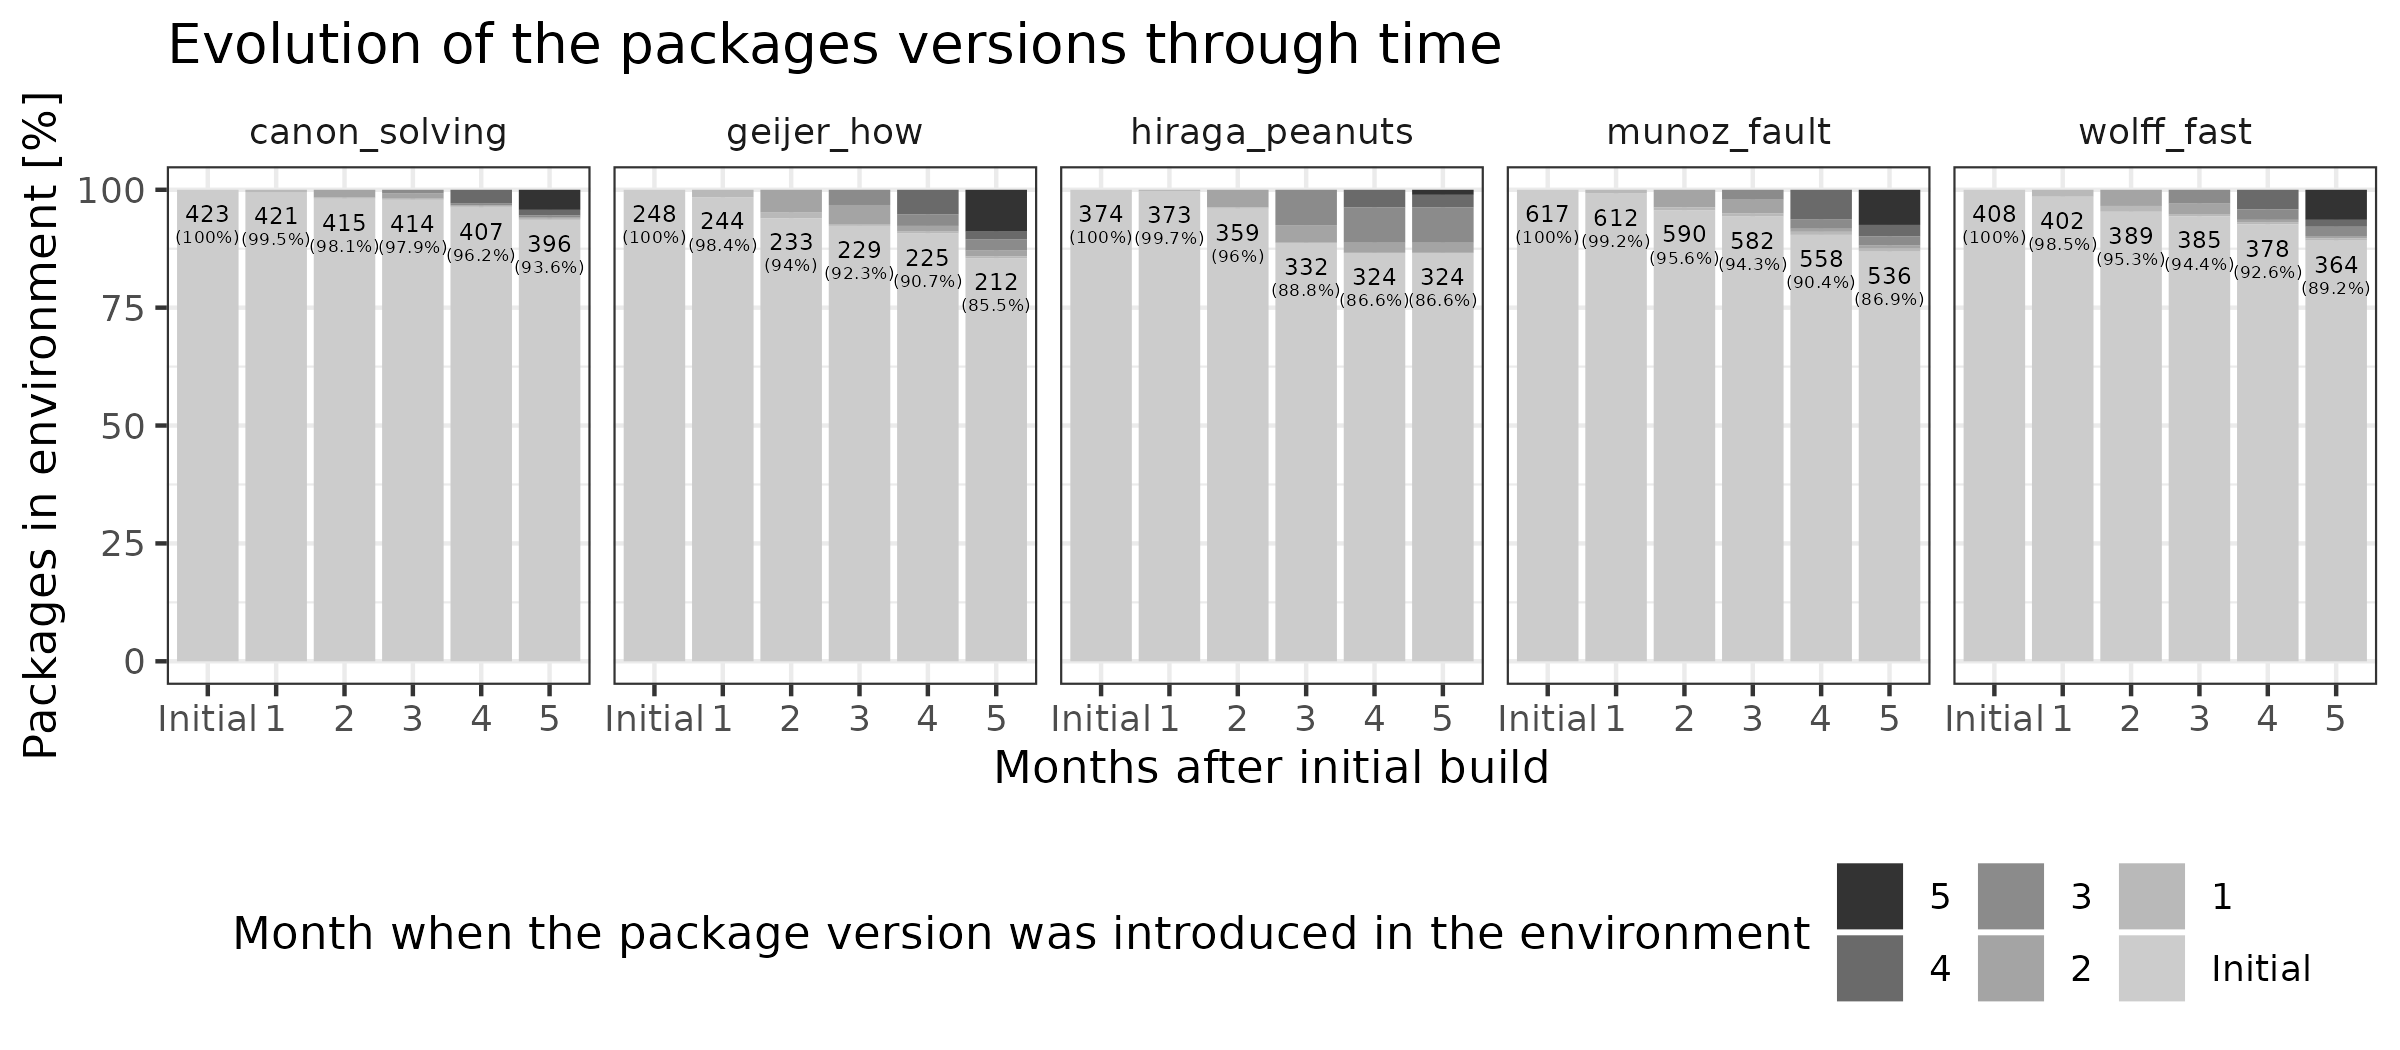
\includegraphics[width=\textwidth]{./fig.pdf}
  \caption{plop}
\end{figure*}


\newpage
\section{Conclusion and Perspectives}

\paragraph{Threats to validity}
Very small sample, only Docker.

\paragraph{Conclusion}

\texttt{Dockerfile}s are not solutions to capture on the long term the software environment.
There is a trade-off between storing the Docker images built by the authors and their recipe.
Use Nix/Guix + Software Heritage.

Even if we only looked at \df s, this study could be extended to other technologies (Apptainer, virtual machines), but it was shown in \cite{guilloteau2024longevity} that \df s was the main solution to provided virtualized software environments.

In this paper, we presented the initial design of our framework to evaluate the longevity of the software environments generated with \df s from research artifacts.

\paragraph{Perspectives}

More

%
% /////////////////////////////////////////////////////////////////////////////////////////////////////

\section*{Acknowledgments}

TODO

%% PAPER ENDS HERE -----------------------------------------------------------------------------------------------

\newpage
%\bibliographystyle{sty/ACM-Reference-Format}
%\bibliography{references}
\printbibliography

\end{document}
